
\documentclass[a4wide]{article}

\def\modulecode{COMP3811}
\def\modulename{Computer Graphics}
\def\editorsuggestion{gedit}

%\input{mymacros}
\usepackage{hyperref}

\setlength{\textheight}{8.3in}
\setlength{\topmargin}{-0.4in}
\setlength{\textwidth}{5.5in}
\setlength{\oddsidemargin}{0.3in}
\setlength{\evensidemargin}{0.3in}

\usepackage{amsmath}
\usepackage{graphicx}
\usepackage{txfonts}
\usepackage{url}
\usepackage{color}
\usepackage{hyperref}

\title{\modulecode: \modulename\\
         Block 1: Tutorial  2\\
       Trigonometry Recap}

\author{Marc de Kamps}
\date{\today}

\begin{document}

\maketitle
\section*{Objective}
In this module you will use a considerable amount of trigonometry. It may have been a while since you've seen trigonometry, and 
in secondary school some results will not have been proven rigorously. In this tutorial, we will review the basic trig functions
and prove the sine rule, the cosine rule, the Pythagorean Theorem. We will derive an important relationship between the scalar product of two vectors
and the angle between them, and introduce the cross product of two vectors. 

It is not the intention to insult anyone's intelligence and attendance for this tutorial will not be monitored, but you will need to make sure you are completely familiar
with these results: in particular I will expect that you can prove each result.

\section*{Definitions}
Just for reference, here are the definitions of the three most important trig functions:
\begin{figure}[h]
  \begin{center}
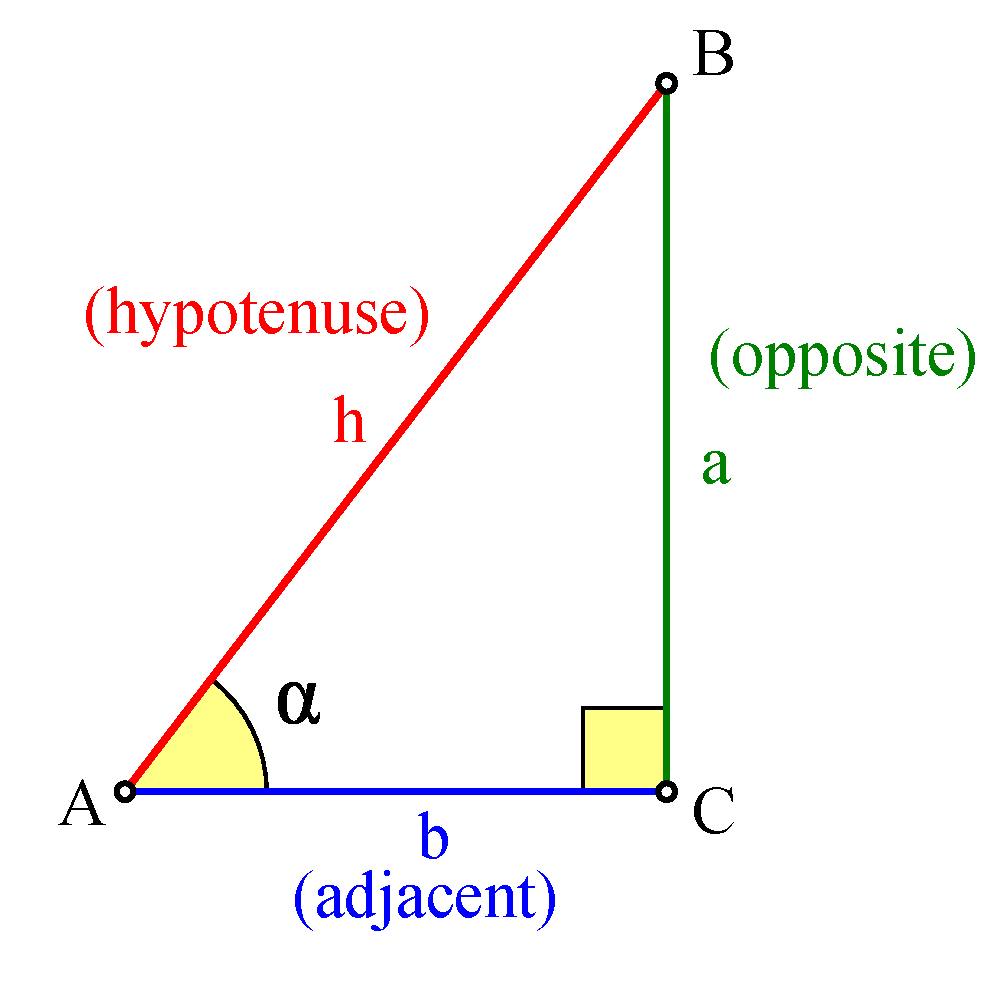
\includegraphics[width=0.4\textwidth]{Trigono_sine_en2.pdf}
  \end{center}
  \caption{Definition of triangle sides.}
  \label{fig-rh}
\end{figure}
Given a right-angled triangle (Fig. \ref{fig-rh}) the sine of angle $\alpha$ is defined as the ratio of the opposite over the hypotenuse, and the cosine as the ratio of the adjacent over the
hypotenuse:
\begin{align}
  \sin \alpha = \frac{a}{h} \\ \nonumber
  \cos \alpha = \frac{b}{h} \nonumber
\end{align}

\section*{The Pythagorean Theorem}
\begin{itemize}
  \item Show that for \emph{any} triangle surfaces area equals half times base times height
\end{itemize}
Consider Fig. \ref{fig-pyth}. 
\begin{figure}[h]
  \begin{center}
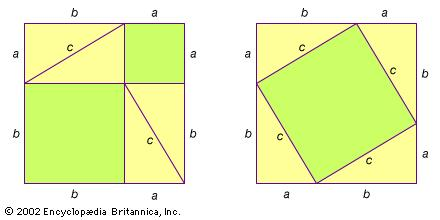
\includegraphics[width=0.4\textwidth]{pyth.jpg}
  \end{center}
  \caption{Set up for a geometrical proof of the Pythagorean Theorem.}
  \label{fig-pyth}
\end{figure}
\begin{itemize}
  \item Find an algebraic expression for the area of the large square.
  \item Find an algebraic expression for the area of one of the triangles.
  \item  Use both expressions to find an algebraic expression for the area of the small square.
  \item Observe that you have now a proof of the Pythagorean Theorem. Explain this carefully.
\end{itemize}

\section*{Cosine and Sine Rule}
The cosine rule can be considered to be a generalization of the Pythagorean Theorem.
\begin{figure}[h]
  \begin{center}
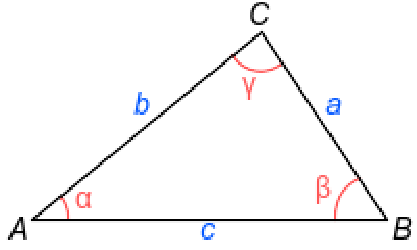
\includegraphics[width=0.4\textwidth]{Triangle_with_notations_2.pdf}
  \end{center}
  \caption{Triangle with notations}
  \label{fig-tri}
\end{figure}
Using the notations from Fig. \ref{fig-tri} the rule is:
$$
a ^2 = b^2 + c^2 - 2bc \cos \alpha
$$
\begin{itemize}
\item Use a symmetry argument to find two other expressions of this rule.
\item Prove the cosine rule. Hint: split the triangle into two right-angled ones; use the Pythagorean Theorem.
\end{itemize}
While you're at it, the sine rule is:
$$
  \sin \alpha/a = \sin \beta/b = \sin \gamma/c
$$

\begin{itemize}
\item Prove the sine rule.
\end{itemize}
\section*{The Scalar Product}
We will speak about vectors in great an gory detail later, but I will assume you are familiar with the basics:
a vector $\vec{a}$ in two dimensions represents a displacement and can be represented by two numbers:
$$
\vec{a} = \left( \begin{array}{c} 1 \\ 3 \end{array} \right)
$$
This can be loosely interpreted as ''\emph{move one to the right and three upwards}''. Vectors can be used to represent
sides from triangles in this way: starting from the origin two vectors $\vec{a}$ and $\vec{b}$ each can represent the
side of a triangle. The length of the side represented by $\vec{a}$ is then given by:
$$
\mid \vec{a} \mid = \sqrt{a^2_x + a^2_y}
$$
where
$$
\vec{a} = \left( \begin{array}{c} a_x \\ a_y \end{array} \right)
$$
So $a_x$ is the so-called $x$-component off $\vec{a}$.

The scalar (or dot)  product is now defined as:
$$
\vec{a} \cdot \vec{b} \equiv a_xb_x + a_yb_y
$$ 

\begin{itemize}
  \item Prove the following relationship using the cosine rule:
\end{itemize}
$$
\vec{a} \cdot \vec{b} = \mid  \vec{a}  \mid \mid \vec{b}  \mid \cos \theta,
$$
where $\theta$ is the angle between vectors $\vec{a}$ and $\vec{b}$.

The dot product can be extended to an arbitrary number of dimensions:
$$
\vec{a} \cdot \vec{b} \equiv \sum^{N}_{J=1} a_j b_j
$$
\begin{itemize}
\item The relationship between dot product and cosine also holds in three and more dimensions. Argue that this suggests that the dot product is invariant under rotations 
(this is in fact true).
\end{itemize}
The dot product is very remarkable: it relates two bags of numbers: (the components of the two vectors; numbers that can be stored, read from file etc.) via
a simple algebraic formula to a geometrical concept: the projection from one vector onto another (Fig. \ref{fig-dot}).

\begin{figure}[h]
  \begin{center}
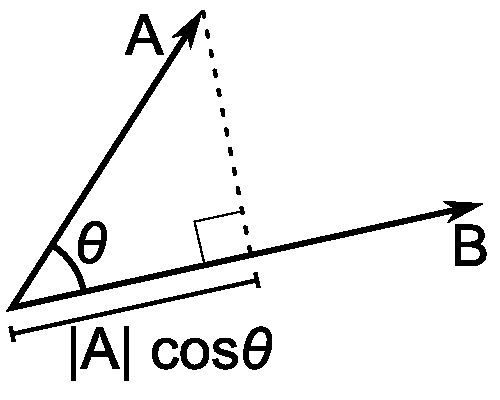
\includegraphics[width=0.4\textwidth]{Dot_Product.pdf}
  \end{center}
  \caption{Projection of one vector onto another via the scalar product}
  \label{fig-dot}
\end{figure}

\begin{itemize}
  \item Find an algebraic expression that relates the components of two vectors that are perpendicular. 
\end{itemize}

\section*{The Cross Product}
The cross product can be defined in two dimensions, but it makes more sense in three dimensions or higher:
let:
$$
\vec{a} = \left( \begin{array}{c} a_1 \\ a_2 \\ a_3 \end{array} \right)
$$
and
$$
\vec{b} = \left( \begin{array}{c} b_1 \\ b_2 \\ b_3 \end{array} \right)
$$
The cross product is another vector defined by:
$$
\vec{a} \times \vec{b} \equiv  \left( \begin{array}{c} a_2 b_3 - a_3 b_2 \\ a_3 b_1 - a_1 b_3 \\ a_1 b_2 - a_2 b_1 \end{array} \right)
$$
It also has a remarkable geometrical interpretation. Consider two vectors $\vec{a}$ and $\vec{b}$ that lie in the $x-y$ plane. So
$$
\vec{a} = \left( \begin{array}{c} a_1 \\ a_2 \\ 0 \end{array} \right)
$$
and
$$
\vec{b} = \left( \begin{array}{c} b_1 \\ b_2 \\ 0 \end{array} \right)
$$
so that the cross product is :
$$
\vec{a} \times \vec{b} \equiv  \left( \begin{array}{c} 0 \\ 0 \\ a_1 b_2 - a_2 b_1 \end{array} \right)
$$

\begin{itemize}
  \item Show that the surface of the parallelogram spanned by $\vec{a}$ and $\vec{b}$  is $\mid a \mid \mid b \mid \sin \theta$.
  \item Show that $a_1 b_2 - a_2b_1 = \mid a \mid \mid b \mid \sin \theta$. \emph{This is a slightly harder question; if you get stuck, move on}
\end{itemize}
Again we find a relationship between the geometrical properties of two vectors and an algebraic expression of its components! Moreover,
one that generalises again (in a way we will explore later) to higher dimensions.


Another interesting property:
\begin{itemize}
  \item Calculate $\vec{a} \cdot (\vec{a} \times \vec{b})$.
  \item Are the brackets necessary?
  \item What do you conclude from the answer?
\end{itemize}


Three dimensional coordinate systems have an orientation: they can be left- or right-handed. We will work mostly in Right-handed coordinate systems, but there
are transformations that change the handedness of a 3D structure.

\begin{itemize}
\item State a transformation that changes handedness
\end{itemize}

There is a visual way for establishing whether a coordinate system is left- or right-handed:

\begin{figure}[h]
  \begin{center}
    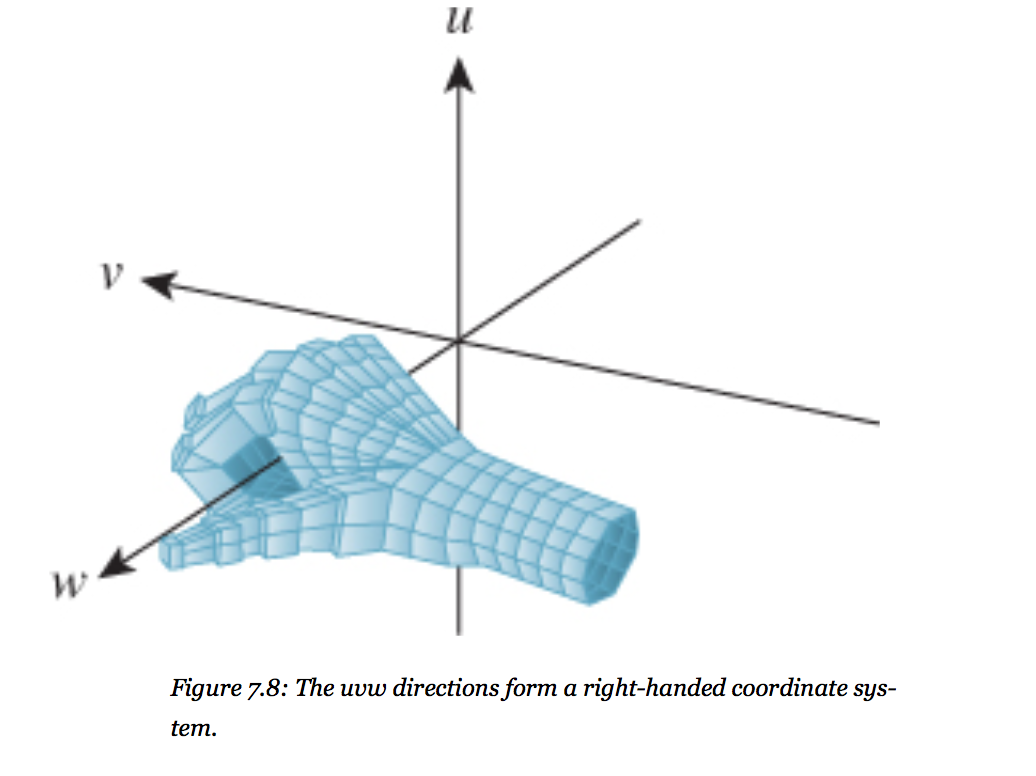
\includegraphics[width=0.7\textwidth]{handedness.png}
  \end{center}
   \caption{ Taken from Hughes \emph{et al.} (Fig. 7.8)}
\end{figure}
Place your little finger (pinky) in the direction of the positive $u$-axis, and curl it in the direction of the positive $v$-axis, closing your fist. If your
thumb points in the direction of the positive $w$-axis, your coordinate system is right-handed, otherwise it is left-handed.


Finally the cross product can be used to establish handedness:
Consider 
$$
\vec{e_x} = \left( \begin{array}{c} 1 \\ 0 \\ 0 \end{array} \right)
$$
and
$$
\vec{e_y} = \left( \begin{array}{c} 0 \\ 1 \\ 0 \end{array} \right)
$$
\begin{itemize}
  \item Calculate $\vec{e_x} \times \vec{e_y}$.
  \item Calculate $\vec{e_y} \times \vec{e_x}$.
  \item Explain the outcome of the last question in terms of the outcome of the penultimate one.
  \item What does the cross product express about handedness?
\end{itemize}
\end{document}
